\subsection{Tx Timestamping interface}
\label{sec:txts}

\begin{figure}[ht]
  \begin{center}
    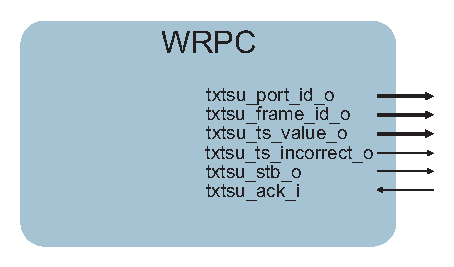
\includegraphics[width=.4\textwidth]{fig/wrpc_txts.pdf}
    \caption{Tx timestamping interface of WRPC}
  \end{center}
\end{figure}

The Tx Timestamping interface provides the timestamps generated inside WRPC for each
Ethernet frame transmitted from user-defined module through the WRF Sink interface.\\

\begin{center}
  \begin{tabular}{|l|l|p{9cm}|}
    \hline
    {\bf Signal name} & {\bf size} & {\bf description} \\
    \hline \hline
    \texttt{txtsu\_port\_id\_o} & 5 & physical port ID from which the timestamp
    was originated. WRPC has only one physical port, so this value is always
    \emph{0}.\\
    \texttt{txtsu\_frame\_id\_o} & 16 & frame ID for which the timestamp is
    available\\
    \texttt{txtsu\_ts\_value\_o} & 32 & Tx timestamp value\\
    \texttt{txtsu\_ts\_incorrect\_o} & 1 & Tx timestamp is not reliable since it
    was generated while PPS generator inside WRPC was being adjusted\\
    \texttt{txtsu\_stb\_o} & 1 & strobe signal that validates the rest of signals
    described above\\
    \texttt{txtsu\_ack\_i} & 1 & acknowledge, indicating that user-defined module
    has received the timestamp\\
    \hline
  \end{tabular}
\end{center}
